\chapter{Results}

% Chapter giving an overview of the numerical results obtained from the implementation

All simulations were carried out on the standard Pitz-Daily backward facing step geometry provided with OpenFOAM. The kinematic viscosity of $\nu=10^{-5}\,\mathrm{m}^2/\mathrm{s}$ and the inlet velocity of $u=10\,\mathrm{m}/\mathrm{s}$ were kept constant for all runs. Using this inlet velocity and the channel width $L=50.8\,\mathrm{mm}$, the Reynolds number of the flow can be approximated as: $$ Re=\frac{uL}{\nu}=50800$$

In order to provide a somewhat objective measure of comparison between the results of the method using different sets of parameters, a vertical line profile of the mean magnitude of the unfiltered velocity field was taken at the location shown in Fig. \ref{fig:line_location} after each run. As well, a simulation using a simple direct solution of the Navier-Stokes equations was performed as a baseline. It must be noted that this is not a true DNS comparison, as the simulation was performed on the same grid as used for all of the following TLES testing, and so is not fine enough to resolve the full range of scales of the system in general. Since such a fully-resolved DNS simulation was prohibitively time-consuming for this project, the under-resolved baseline case was considered acceptable to at least check for any large deviations resulting from the methods being tested, and for simplicity is referred to as DNS in the following analysis. The location of the line was chosen to be at the minimum value of the recirculation vortex in the DNS baseline, so as to have a distinct feature to compare with between runs.

\begin{figure}[!b]
\centering
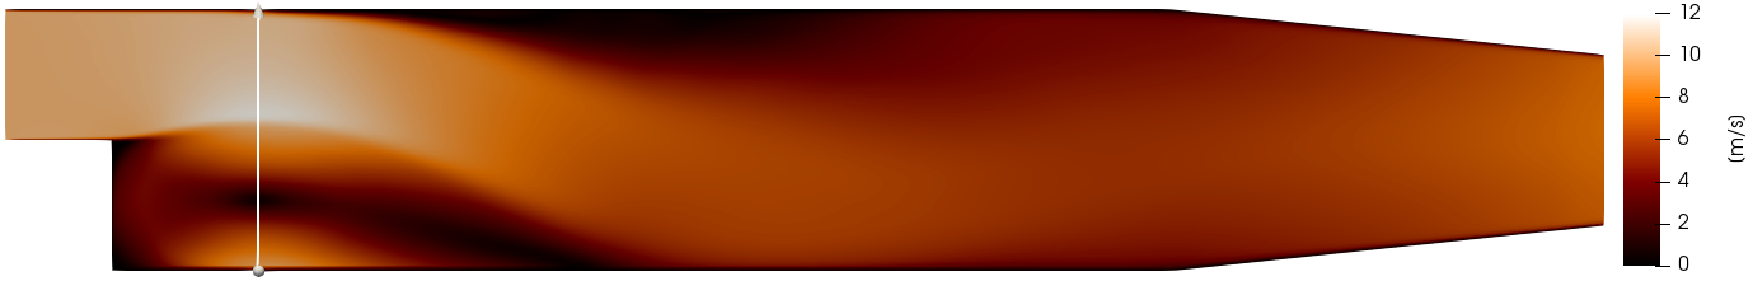
\includegraphics[width=0.75\textwidth]{figures/line_location.pdf}
\caption{Representative image of a $|\bar{u}|_{\mathrm{mean}}$ velocity field with a white line showing the location $x=28.6\,\mathrm{mm}$ past the step at which the comparison profiles were captured}
\label{fig:line_location}
\end{figure}

To start with, several simulations were run using only the basic TLES implementation, with no regularization or DC. This gave one free parameter to be varied, the filter width ratio $r$, and the resulting profiles were taken at an end time of $t_\mathrm{final}=0.1$ using a time step of $\Delta t=10^{-6}$ for all runs. It was observed that the simulation becomes unstable if the filter width is made too large, and so this time step was chosen as it gave a small range of values, up to $r\approx 28$, for which the base method was stable and any effects of varying $r$ in isolation could be observed.

The results of this initial study are shown in Fig. \ref{fig:line_data_no_reg} and the profiles from the various runs are seen to lie almost completely atop one another. This would seem to suggest that the effect of $r$ is minimal within the range of values which are stable without regularization.

\begin{figure}[!htb]
\centering
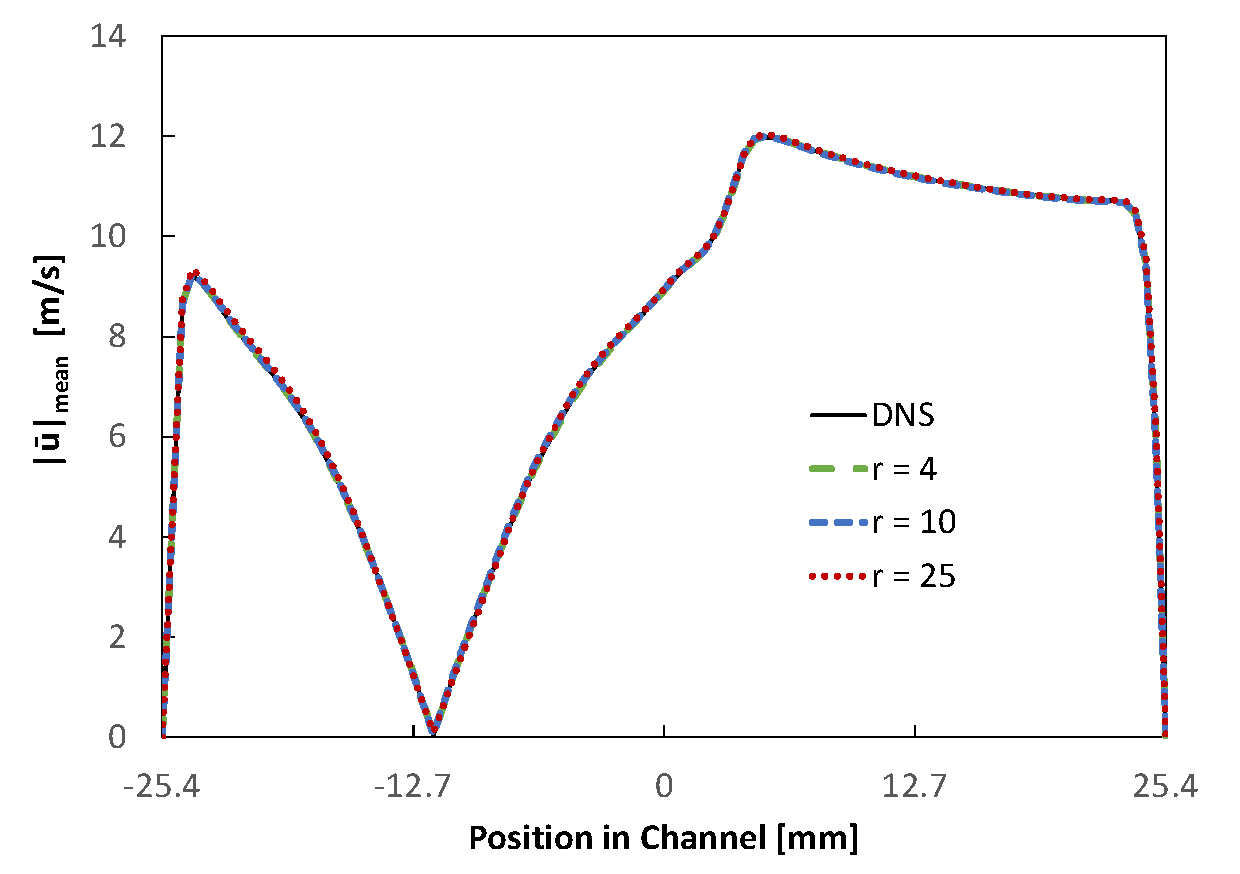
\includegraphics[width=0.75\textwidth]{figures/line_data_no_reg.pdf}
\caption{Comparison of line profiles from the $|\bar{u}|_{\mathrm{mean}}$ velocity field at $x=28.6\,\mathrm{mm}$ for various values of filter width $r$, taken at $t_\mathrm{final}=0.1$ using $\Delta t=10^{-6}$}
\label{fig:line_data_no_reg}
\end{figure}

The effects of adding DC to the method as per the projection method outlined in section \ref{sec:DC} were investigated next. A small increase in the stable range of the filter width $r$ was observed, with the largest stable value for $r$ increasing from $r=4.4$ to $r=4.7$ when $\Delta t=10^{-5}$, and from $r=28$ to $r=29$ for a $\Delta t=10^{-6}$ time step. Simulations were run with DC included in the simulations for the same already stable values of $r$ as in the previous set as well as for the now stabilized $r=29$ case, and the results are shown in Fig. \ref{fig:line_data_DC}. This allowed for potential comparison between the effects of DC both when it was and was not required to achieve stability in the first instance.

Unlike with the base TLES simulations, all of the runs with DC are seen to be no longer as perfectly concident with the baseline simulation, although the deviation is relatively minor and the variations of $r$ still appear to have little discernible impact on the results. Additionally, the runtime of the simulations increased by only between 5-11\% for the values of $r$ with a counterpart simulation not using DC, indicating decent efficiency of the DC implementation using an iterative solver with a relaxed tolerance, as discussed in sections \ref{sec:DC} and \ref{chap:Imp}.

\begin{figure}[!t]
\centering
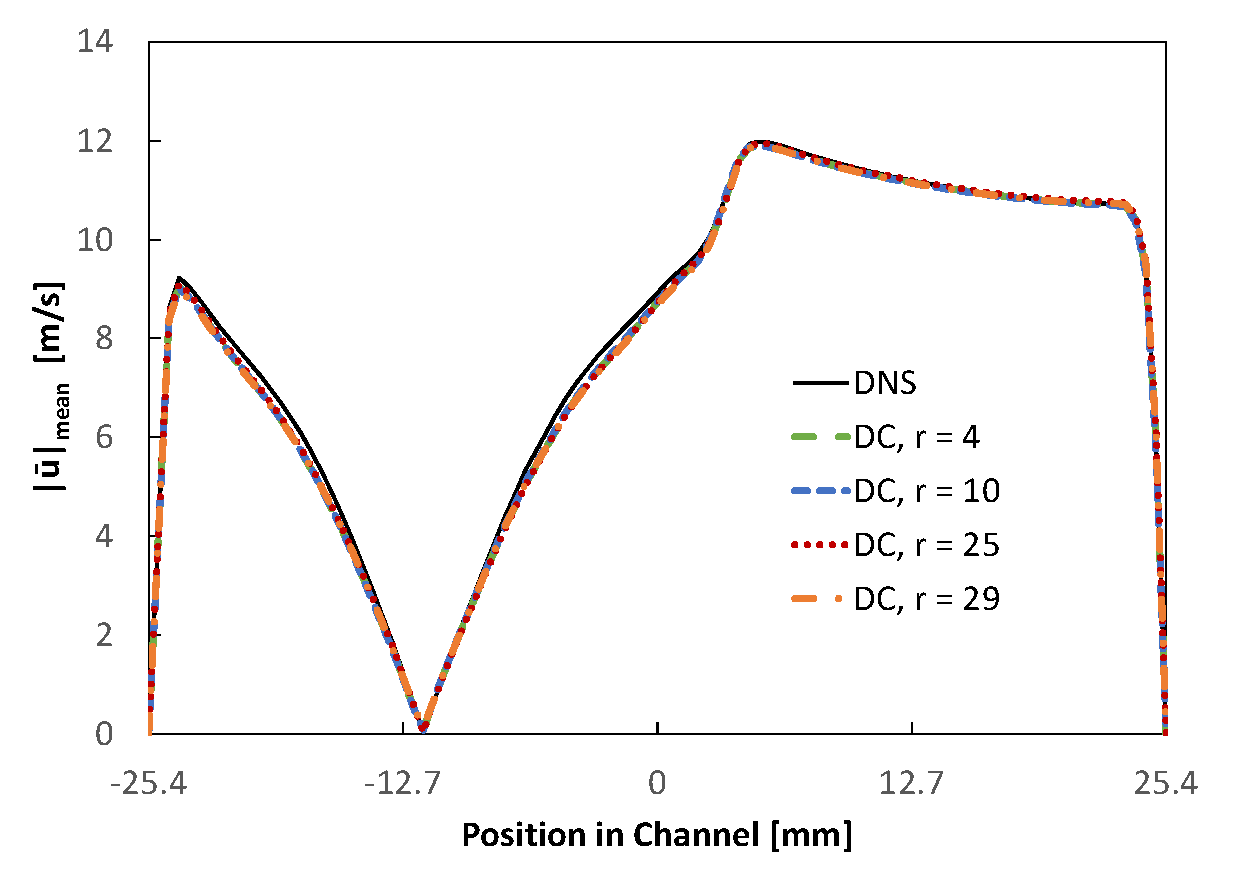
\includegraphics[width=0.75\textwidth]{figures/line_data_DC.pdf}
\caption{Comparison of line profiles from the $|\bar{u}|_{\mathrm{mean}}$ velocity field at $x=28.6\,\mathrm{mm}$ for various values of filter width $r$ with divergence cleaning, taken at $t_\mathrm{final}=0.1$ using $\Delta t=10^{-6}$}
\label{fig:line_data_DC}
\end{figure}

\begin{figure}[!h]
\centering
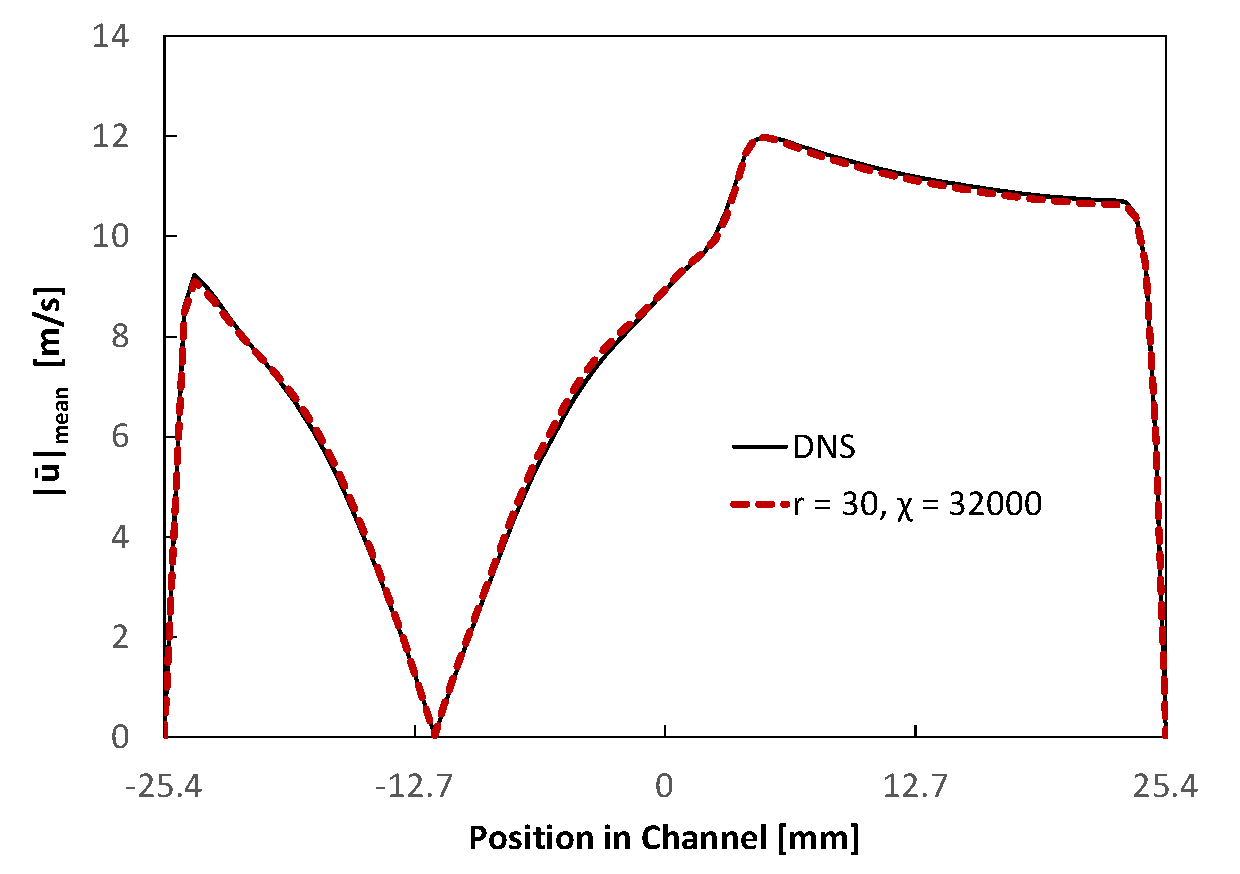
\includegraphics[width=0.75\textwidth]{figures/line_data_reg.pdf}
\caption{Line profile from the $|\bar{u}|_{\mathrm{mean}}$ velocity field at $x=28.6\,\mathrm{mm}$ for $r=30$ with regularization. $\chi = 32000$, $\tilde{r}=100$, $t_\mathrm{final}=0.1$, and $\Delta t=10^{-6}$}
\label{fig:line_data_reg}
\end{figure}

In Fig. \ref{fig:line_data_reg} is shown the result of a run at $r=30$, using regularization with a control value of $\chi=32000$ to stabilize the simulation. This value of $\chi$ was chosen so as to be slightly larger than the minimal value for which the simulation was found to be stable for $r=30$, as discussed later in this chapter. It is observed that while the shape of the profile is very similar to the baseline case, the data shown was collected after propogating the simulation through 87X as many timesteps, to a $t_\mathrm{final}=8.4$ compared to $0.1$ for the baseline (and all other profiles shown.) The final time for comparison was chosen to be the time when the minimum of the recirculation vortex in the regularized run reached the same location as in the compared against baseline profile. Such good agreement between the profiles when matching such a recognizable feature as the vortex minimum suggests that the regularization stabilized simulation seems to evolve through the same sequence as without regularization, only at a \emph{much} slower rate.

Since most cases of instability in the simulation manifested within the first few dozen time steps (approx. 30-40 or less), and given the large number of parameter sets that needed to be tested, for the purposes of the following section a simulation was considered `stable' if it ran for 100 timesteps without failing. It is noted that a small number of the runs performed crashed even after 80+ timesteps, so this 100 timestep rule is certainly not an ironclad guarantee of stability over a much longer run. However, as in all of these cases it was the transition from stable to unstable that was under investigation, it suffices to warn that the reported minimal $\chi$ values required for stability should be regarded as providing only marginal stability, and slightly larger values might be safer in a real simulations to provide some margin of safety.

\begin{figure}[!tb]
\centering
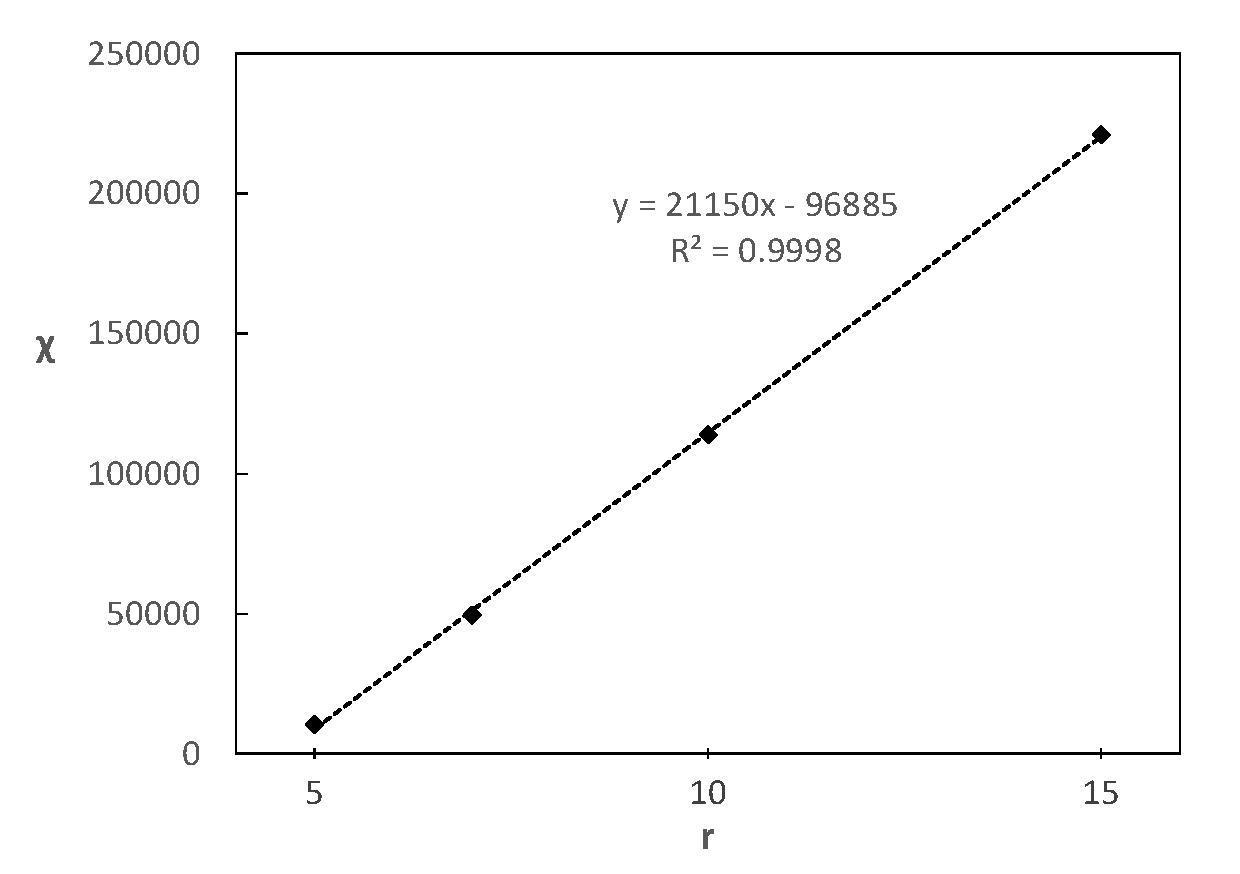
\includegraphics[width=0.75\textwidth]{figures/min_chi_dt5_r100.pdf}
\caption{Minimum $\chi$ values required to stabilize simulation for various values of $r$, using $\Delta t=10^{-5}$ and $\tilde{r}=100$, and showing the linear least squares line regression}
\label{fig:min_chi_dt5_r100}
\end{figure}

\begin{figure}[!tb]
\centering
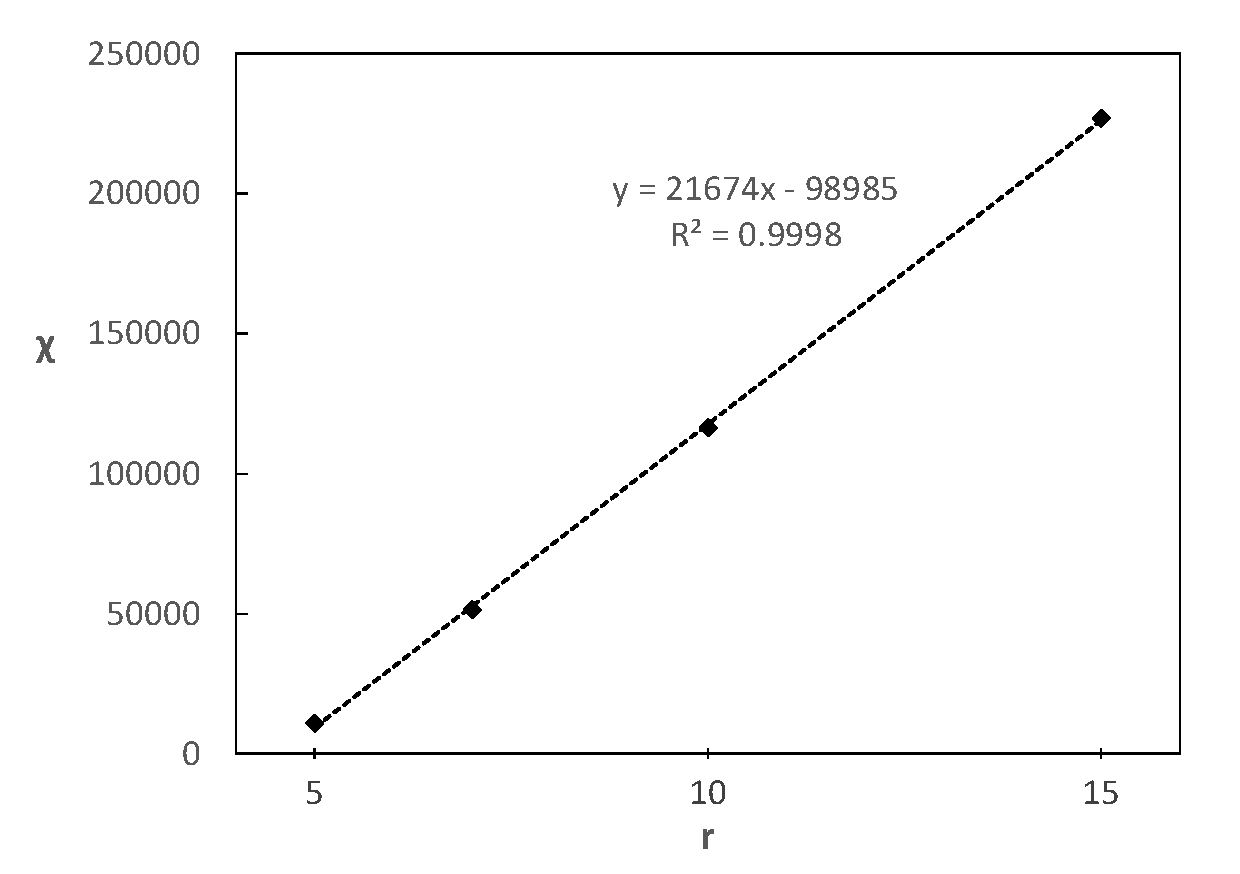
\includegraphics[width=0.75\textwidth]{figures/min_chi_dt5_r10.pdf}
\caption{Minimum $\chi$ values required to stabilize simulation for various values of $r$, using $\Delta t=10^{-5}$ and $\tilde{r}=10$, and showing the linear least squares line regression}
\label{fig:min_chi_dt5_r10}
\end{figure}

\begin{figure}[!tb]
\centering
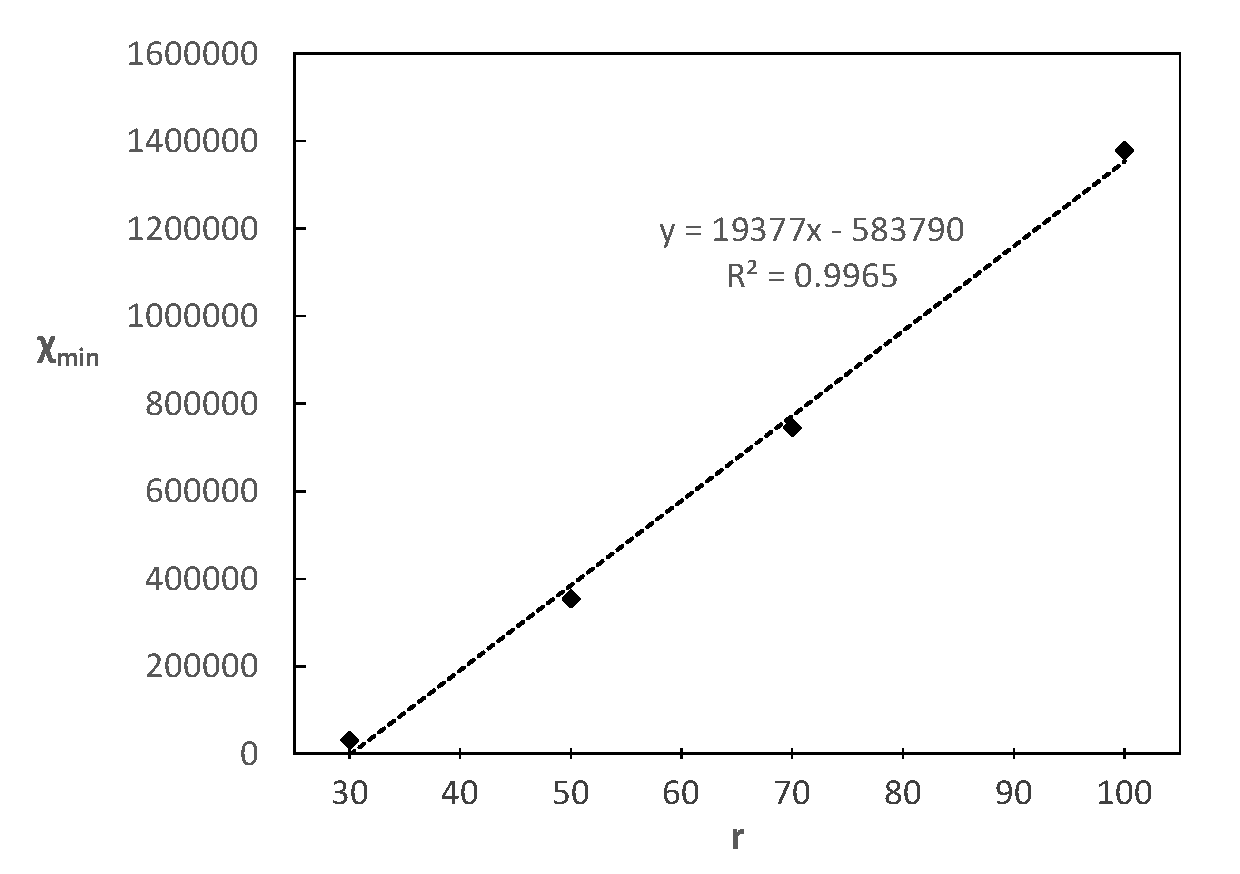
\includegraphics[width=0.75\textwidth]{figures/min_chi_dt6_r100.pdf}
\caption{Minimum $\chi$ values required to stabilize simulation for various values of $r$, using $\Delta t=10^{-6}$ and $\tilde{r}=100$, and showing the linear least squares line regression}
\label{fig:min_chi_dt6_r100}
\end{figure}
